\chapter{Monodromy groups of rank 4}

\section{Two 4-transpositions}
\label{rank4-2-4transpositions}

\subsection{Two double edges}
\label{rank4-2-1-4transpositions}

\subsubsection{Length 8}

\begin{figure}[H]
  \begin{center}
    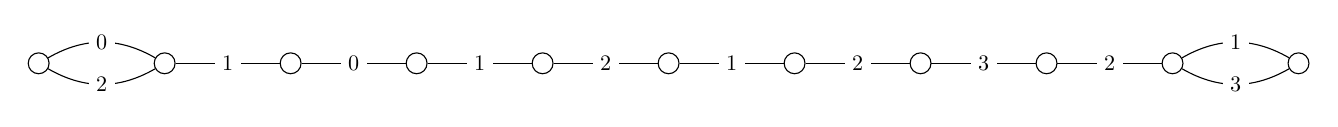
\begin{tikzpicture}[scale=.8]

      \begin{scope}[every node/.style={circle,draw, transform shape}]
        \node (1)  at (0,0) {};
        \node (2)  at (2,0) {};
        \node (3)  at (4,0) {};
        \node (4)  at (6,0)  {};
        \node (5)  at (8,0)  {};
        \node (6)  at (10,0)  {};
        \node (7)  at (12,0)  {};
        \node (8)  at (18,0)  {};
        \node (9)  at (20,0)  {};
        \node (10) at (16,0)  {};
        \node (11) at (14,0)  {};
      \end{scope}

      \begin{scope}[every node/.style={fill=white, transform shape}]

        \begin{scope}[every edge/.style={draw}]
          \path (1)  edge[bend left=30] node {$0$} (2);
          \path (3)  edge node {$0$} (4);
          \path (2)  edge node {$1$} (3);
          \path (4)  edge node {$1$} (5);
          \path (6)  edge node {$1$} (7);
          \path (8)  edge[bend left=30] node {$1$} (9);
          \path (1)  edge[bend right=30] node {$2$} (2);
          \path (5)  edge node {$2$} (6);
          \path (7)  edge node {$2$} (11);
          \path (8)  edge node {$2$} (10);
          \path (8)  edge[bend right=30] node {$3$} (9);
          \path (10) edge node {$3$} (11);
        \end{scope}
      \end{scope}

    \end{tikzpicture}
    \caption{}
    \label{r4-1-1}
  \end{center}
\end{figure}

\begin{figure}[H]
  \begin{center}
    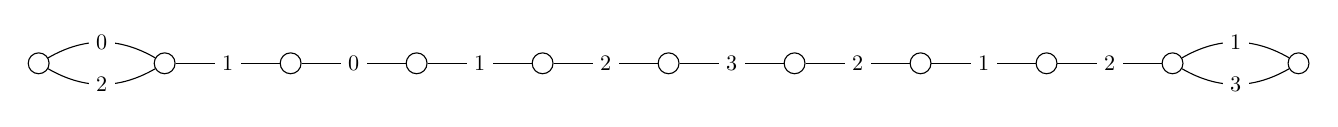
\begin{tikzpicture}[scale=.8]

      \begin{scope}[every node/.style={circle,draw, transform shape}]
        \node (1)  at (0,0) {};
        \node (2)  at (2,0) {};
        \node (3)  at (4,0) {};
        \node (4)  at (6,0)  {};
        \node (5)  at (8,0)  {};
        \node (6)  at (20,0)  {};
        \node (7)  at (18,0)  {};
        \node (8)  at (16,0)  {};
        \node (9)  at (14,0)  {};
        \node (10) at (10,0)  {};
        \node (11) at (12,0)  {};
      \end{scope}

      \begin{scope}[every node/.style={fill=white, transform shape}]

        \begin{scope}[every edge/.style={draw}]
          \path (1)  edge[bend left=30] node {$0$} (2);
          \path (3)  edge node {$0$} (4);
          \path (2)  edge node {$1$} (3);
          \path (4)  edge node {$1$} (5);
          \path (6)  edge[bend right=30] node {$1$} (7);
          \path (8)  edge node {$1$} (9);
          \path (1)  edge[bend right=30] node {$2$} (2);
          \path (5)  edge node {$2$} (10);
          \path (7)  edge node {$2$} (8);
          \path (9)  edge node {$2$} (11);
          \path (6)  edge[bend left=30] node {$3$} (7);
          \path (10) edge node {$3$} (11);
        \end{scope}
      \end{scope}

    \end{tikzpicture}
    \caption{}
    \label{r4-1-2}
  \end{center}
\end{figure}

\begin{figure}[H]
  \begin{center}
    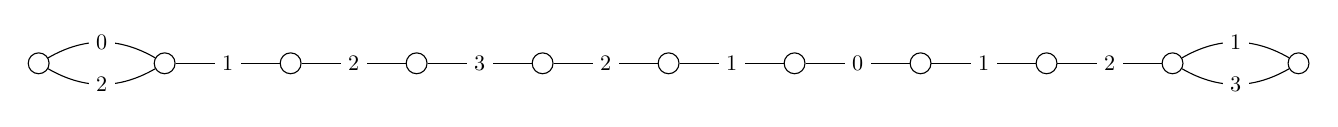
\begin{tikzpicture}[scale=.8]

      \begin{scope}[every node/.style={circle,draw, transform shape}]
        \node (1)  at (14,0) {};
        \node (2)  at (12,0)  {};
        \node (3)  at (2,0)  {};
        \node (4)  at (0,0)  {};
        \node (5)  at (6,0)  {};
        \node (6)  at (8,0)  {};
        \node (7)  at (10,0)  {};
        \node (8)  at (16,0)  {};
        \node (9)  at (18,0)  {};
        \node (10) at (20,0)  {};
        \node (11) at (4,0) {};
      \end{scope}

      \begin{scope}[every node/.style={fill=white, transform shape}]

        \begin{scope}[every edge/.style={draw}]
          \path (1)  edge node {$0$} (2);
          \path (3)  edge[bend right=30] node {$0$} (4);
          \path (1)  edge node {$1$} (8);
          \path (2)  edge node {$1$} (7);
          \path (3)  edge node {$1$} (11);
          \path (9)  edge[bend left=30] node {$1$} (10);
          \path (3)  edge[bend left=30] node {$2$} (4);
          \path (5)  edge node {$2$} (11);
          \path (6)  edge node {$2$} (7);
          \path (8)  edge node {$2$} (9);
          \path (5)  edge node {$3$} (6);
          \path (9)  edge[bend right=30] node {$3$} (10);
        \end{scope}
      \end{scope}

    \end{tikzpicture}
    \caption{}
    \label{r4-1-3}
  \end{center}
\end{figure}

\subsubsection{Length 6}

\begin{figure}[H]
  \begin{center}
    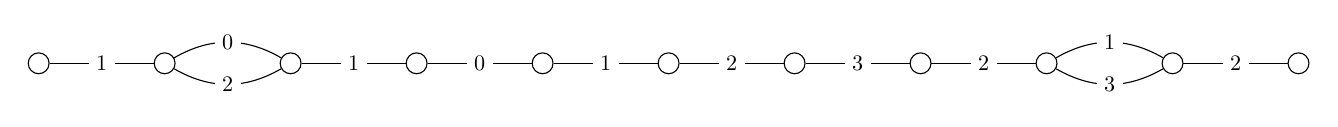
\begin{tikzpicture}[scale=.8]

      \begin{scope}[every node/.style={circle,draw, transform shape}]
        \node (1)  at (2,0)  {};
        \node (2)  at (4,0)  {};
        \node (3)  at (6,0)  {};
        \node (4)  at (8,0)  {};
        \node (5)  at (10,0)  {};
        \node (6)  at (12,0)  {};
        \node (7)  at (14,0)  {};
        \node (8)  at (20,0) {};
        \node (9)  at (18,0)  {};
        \node (10) at (16,0) {};
        \node (11) at (0,0) {};
      \end{scope}

      \begin{scope}[every node/.style={fill=white, transform shape}]

        \begin{scope}[every edge/.style={draw}]
          \path (1)  edge[bend left=30] node {$0$} (2);
          \path (3)  edge node {$0$} (4);
          \path (1)  edge node {$1$} (11);
          \path (2)  edge node {$1$} (3);
          \path (4)  edge node {$1$} (5);
          \path (9)  edge[bend right=30] node {$1$} (10);
          \path (1)  edge[bend right=30] node {$2$} (2);
          \path (5)  edge node {$2$} (6);
          \path (7)  edge node {$2$} (10);
          \path (8)  edge node {$2$} (9);
          \path (6)  edge node {$3$} (7);
          \path (9)  edge[bend left=30] node {$3$} (10);
        \end{scope}
      \end{scope}

    \end{tikzpicture}
    \caption{}
    \label{r4-1-4}
  \end{center}
\end{figure}


\begin{figure}[H]
  \begin{center}
    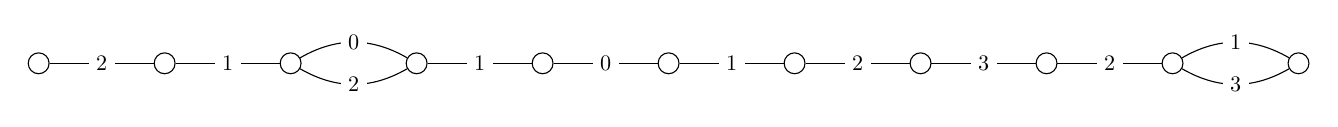
\begin{tikzpicture}[scale=.8]

      \begin{scope}[every node/.style={circle,draw, transform shape}]
        \node (1)  at (10,0)  {};
        \node (2)  at (8,0)  {};
        \node (3)  at (6,0)  {};
        \node (4)  at (4,0)  {};
        \node (5)  at (2,0) {};
        \node (6)  at (0,0)  {};
        \node (7)  at (14,0) {};
        \node (8)  at (16,0)  {};
        \node (9)  at (20,0)  {};
        \node (10) at (18,0) {};
        \node (11) at (12,0) {};
      \end{scope}

      \begin{scope}[every node/.style={fill=white, transform shape}]

        \begin{scope}[every edge/.style={draw}]
          \path (1)  edge node {$0$} (2);
          \path (3)  edge[bend right=30] node {$0$} (4);
          \path (1)  edge node {$1$} (11);
          \path (2)  edge node {$1$} (3);
          \path (4)  edge node {$1$} (5);
          \path (9)  edge[bend right=30] node {$1$} (10);
          \path (3)  edge[bend left=30] node {$2$} (4);
          \path (5)  edge node {$2$} (6);
          \path (7)  edge node {$2$} (11);
          \path (8)  edge node {$2$} (10);
          \path (7)  edge node {$3$} (8);
          \path (9)  edge[bend left=30] node {$3$} (10);
        \end{scope}
      \end{scope}

    \end{tikzpicture}
    \caption{}
    \label{r4-1-5}
  \end{center}
\end{figure}

\begin{figure}[H]
  \begin{center}
    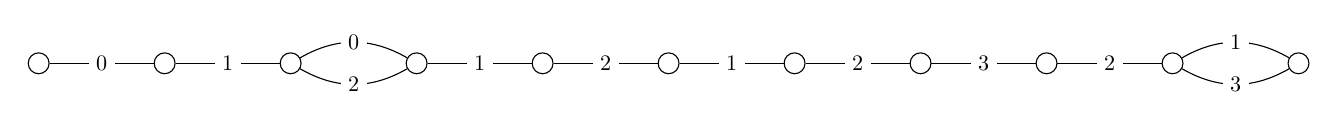
\begin{tikzpicture}[scale=.8]

      \begin{scope}[every node/.style={circle,draw, transform shape}]
        \node (1)  at (20,0) {};
        \node (2)  at (18,0) {};
        \node (3)  at (16,0) {};
        \node (4)  at (14,0)  {};
        \node (5)  at (12,0)  {};
        \node (6)  at (10,0)  {};
        \node (7)  at (8,0)  {};
        \node (8)  at (6,0)  {};
        \node (9)  at (4,0)  {};
        \node (10) at (2,0)  {};
        \node (11) at (0,0)  {};
      \end{scope}

      \begin{scope}[every node/.style={fill=white, transform shape}]

        \begin{scope}[every edge/.style={draw}]
          \path (1)  edge[bend left=30] node {$3$} (2);
          \path (3)  edge node {$3$} (4);
          \path (2)  edge node {$2$} (3);
          \path (4)  edge node {$2$} (5);
          \path (6)  edge node {$2$} (7);
          \path (8)  edge[bend left=30] node {$2$} (9);
          \path (1)  edge[bend right=30] node {$1$} (2);
          \path (5)  edge node {$1$} (6);
          \path (7)  edge node {$1$} (8);
          \path (9)  edge node {$1$} (10);
          \path (8)  edge[bend right=30] node {$0$} (9);
          \path (10) edge node {$0$} (11);
        \end{scope}
      \end{scope}

    \end{tikzpicture}
    \caption{}
    \label{r4-1-6}
  \end{center}
\end{figure}

\begin{figure}[H]
  \begin{center}
    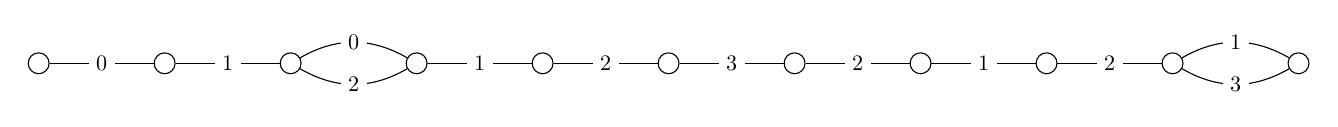
\begin{tikzpicture}[scale=.8]

      \begin{scope}[every node/.style={circle,draw, transform shape}]
        \node (1)  at (0,0) {};
        \node (2)  at (2,0) {};
        \node (3)  at (4,0) {};
        \node (4)  at (6,0)  {};
        \node (5)  at (8,0)  {};
        \node (6)  at (20,0)  {};
        \node (7)  at (18,0)  {};
        \node (8)  at (16,0)  {};
        \node (9)  at (14,0)  {};
        \node (10) at (12,0)  {};
        \node (11) at (10,0)  {};
      \end{scope}

      \begin{scope}[every node/.style={fill=white, transform shape}]

        \begin{scope}[every edge/.style={draw}]
          \path (1)  edge node {$0$} (2);
          \path (3)  edge[bend left=30] node {$0$} (4);
          \path (2)  edge node {$1$} (3);
          \path (4)  edge node {$1$} (5);
          \path (6)  edge[bend right=30] node {$1$} (7);
          \path (8)  edge node {$1$} (9);
          \path (3)  edge[bend right=30] node {$2$} (4);
          \path (5)  edge node {$2$} (11);
          \path (7)  edge node {$2$} (8);
          \path (9)  edge node {$2$} (10);
          \path (6)  edge[bend left=30] node {$3$} (7);
          \path (10) edge node {$3$} (11);
        \end{scope}
      \end{scope}

    \end{tikzpicture}
    \caption{}
    \label{r4-1-7}
  \end{center}
\end{figure}

\subsubsection{Length 4}

\begin{figure}[H]
  \begin{center}
    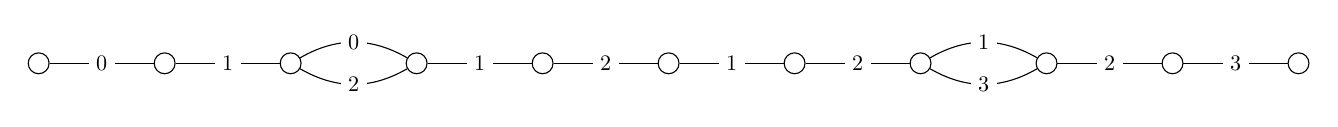
\begin{tikzpicture}[scale=.8]

      \begin{scope}[every node/.style={circle,draw, transform shape}]
        \node (1)  at (0,0) {};
        \node (2)  at (2,0) {};
        \node (3)  at (4,0) {};
        \node (4)  at (6,0)  {};
        \node (5)  at (8,0)  {};
        \node (6)  at (10,0)  {};
        \node (7)  at (12,0)  {};
        \node (8)  at (14,0)  {};
        \node (9)  at (16,0)  {};
        \node (10) at (18,0)  {};
        \node (11) at (20,0)  {};
      \end{scope}

      \begin{scope}[every node/.style={fill=white, transform shape}]

        \begin{scope}[every edge/.style={draw}]
          \path (1)  edge node {$0$} (2);
          \path (3)  edge[bend left=30] node {$0$} (4);
          \path (2)  edge node {$1$} (3);
          \path (4)  edge node {$1$} (5);
          \path (6)  edge node {$1$} (7);
          \path (8)  edge[bend left=30] node {$1$} (9);
          \path (3)  edge[bend right=30] node {$2$} (4);
          \path (5)  edge node {$2$} (6);
          \path (7)  edge node {$2$} (8);
          \path (9)  edge node {$2$} (10);
          \path (8)  edge[bend right=30] node {$3$} (9);
          \path (10) edge node {$3$} (11);
        \end{scope}
      \end{scope}

    \end{tikzpicture}
    \caption{}
    \label{r4-1-8}
  \end{center}
\end{figure}

\begin{figure}[H]
  \begin{center}
    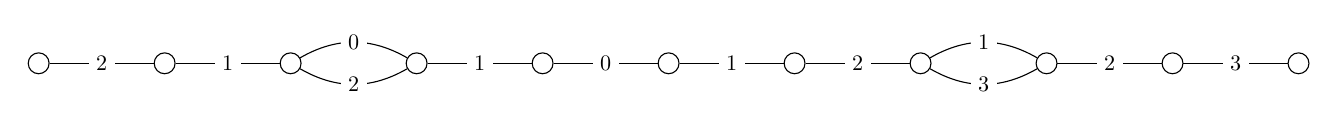
\begin{tikzpicture}[scale=.8]

      \begin{scope}[every node/.style={circle,draw, transform shape}]
        \node (1)  at (10,0)  {};
        \node (2)  at (8,0)  {};
        \node (3)  at (6,0)  {};
        \node (4)  at (4,0)  {};
        \node (5)  at (2,0) {};
        \node (6)  at (20,0) {};
        \node (7)  at (0,0) {};
        \node (8)  at (18,0)  {};
        \node (9)  at (16,0)  {};
        \node (10) at (14,0) {};
        \node (11) at (12,0) {};
      \end{scope}

      \begin{scope}[every node/.style={fill=white, transform shape}]

        \begin{scope}[every edge/.style={draw}]
          \path (1)  edge node {$0$} (2);
          \path (3)  edge[bend right=30] node {$0$} (4);
          \path (1)  edge node {$1$} (11);
          \path (2)  edge node {$1$} (3);
          \path (4)  edge node {$1$} (5);
          \path (9)  edge[bend right=30] node {$1$} (10);
          \path (3)  edge[bend left=30] node {$2$} (4);
          \path (5)  edge node {$2$} (7);
          \path (8)  edge node {$2$} (9);
          \path (10) edge node {$2$} (11);
          \path (6)  edge node {$3$} (8);
          \path (9)  edge[bend left=30] node {$3$} (10);
        \end{scope}
      \end{scope}

    \end{tikzpicture}
    \caption{}
    \label{r4-1-9}
  \end{center}
\end{figure}

\begin{figure}[H]
  \begin{center}
    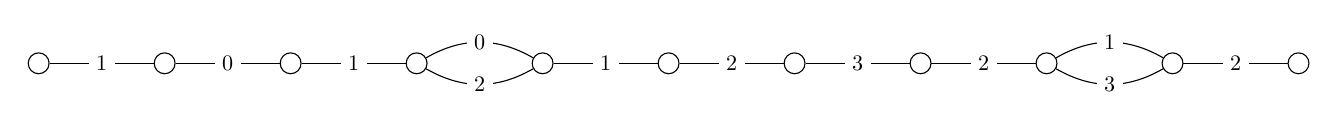
\begin{tikzpicture}[scale=.8]

      \begin{scope}[every node/.style={circle,draw, transform shape}]
        \node (1)  at (8,0)  {};
        \node (2)  at (6,0)  {};
        \node (3)  at (4,0)  {};
        \node (4)  at (2,0)  {};
        \node (5)  at (0,0)  {};
        \node (6)  at (12,0)  {};
        \node (7)  at (14,0)  {};
        \node (8)  at (20,0) {};
        \node (9)  at (18,0)  {};
        \node (10) at (16,0) {};
        \node (11) at (10,0) {};
      \end{scope}

      \begin{scope}[every node/.style={fill=white, transform shape}]

        \begin{scope}[every edge/.style={draw}]
          \path (1)  edge[bend right=30] node {$0$} (2);
          \path (3)  edge node {$0$} (4);
          \path (1)  edge node {$1$} (11);
          \path (2)  edge node {$1$} (3);
          \path (4)  edge node {$1$} (5);
          \path (9)  edge[bend right=30] node {$1$} (10);
          \path (1)  edge[bend left=30] node {$2$} (2);
          \path (6)  edge node {$2$} (11);
          \path (7)  edge node {$2$} (10);
          \path (8)  edge node {$2$} (9);
          \path (6)  edge node {$3$} (7);
          \path (9)  edge[bend left=30] node {$3$} (10);
        \end{scope}
      \end{scope}

    \end{tikzpicture}
    \caption{}
    \label{r4-1-10}
  \end{center}
\end{figure}

\begin{figure}[H]
  \begin{center}
    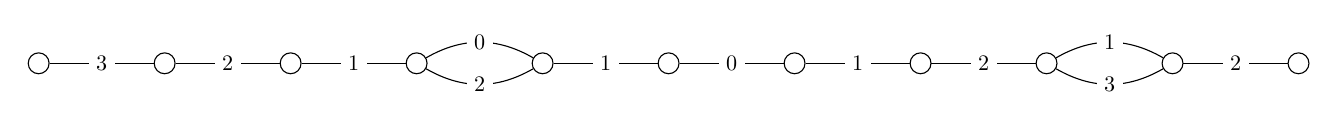
\begin{tikzpicture}[scale=.8]

      \begin{scope}[every node/.style={circle,draw, transform shape}]
        \node (1)  at (12,0)  {};
        \node (2)  at (10,0)  {};
        \node (3)  at (8,0)  {};
        \node (4)  at (6,0)  {};
        \node (5)  at (4,0) {};
        \node (6)  at (2,0)  {};
        \node (7)  at (0,0)  {};
        \node (8)  at (20,0)  {};
        \node (9)  at (18,0)  {};
        \node (10) at (16,0) {};
        \node (11) at (14,0) {};
      \end{scope}

      \begin{scope}[every node/.style={fill=white, transform shape}]

        \begin{scope}[every edge/.style={draw}]
          \path (1)  edge node {$0$} (2);
          \path (3)  edge[bend right=30] node {$0$} (4);
          \path (1)  edge node {$1$} (11);
          \path (2)  edge node {$1$} (3);
          \path (4)  edge node {$1$} (5);
          \path (9)  edge[bend right=30] node {$1$} (10);
          \path (3)  edge[bend left=30] node {$2$} (4);
          \path (5)  edge node {$2$} (6);
          \path (8)  edge node {$2$} (9);
          \path (10) edge node {$2$} (11);
          \path (6)  edge node {$3$} (7);
          \path (9)  edge[bend left=30] node {$3$} (10);
        \end{scope}
      \end{scope}

    \end{tikzpicture}
    \caption{}
    \label{r4-1-11}
  \end{center}
\end{figure}

\begin{figure}[H]
  \begin{center}
    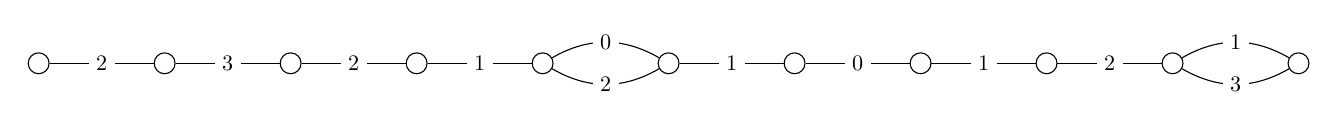
\begin{tikzpicture}[scale=.8]

      \begin{scope}[every node/.style={circle,draw, transform shape}]
        \node (1)  at (14,0)  {};
        \node (2)  at (12,0)  {};
        \node (3)  at (10,0)  {};
        \node (4)  at (8,0)  {};
        \node (5)  at (6,0) {};
        \node (6)  at (4,0) {};
        \node (7)  at (2,0) {};
        \node (8)  at (0,0)  {};
        \node (9)  at (20,0)  {};
        \node (10) at (18,0) {};
        \node (11) at (16,0) {};
      \end{scope}

      \begin{scope}[every node/.style={fill=white, transform shape}]

        \begin{scope}[every edge/.style={draw}]
          \path (1)  edge node {$0$} (2);
          \path (3)  edge[bend right=30] node {$0$} (4);
          \path (1)  edge node {$1$} (11);
          \path (2)  edge node {$1$} (3);
          \path (4)  edge node {$1$} (5);
          \path (9)  edge[bend right=30] node {$1$} (10);
          \path (3)  edge[bend left=30] node {$2$} (4);
          \path (5)  edge node {$2$} (6);
          \path (7)  edge node {$2$} (8);
          \path (10) edge node {$2$} (11);
          \path (6)  edge node {$3$} (7);
          \path (9)  edge[bend left=30] node {$3$} (10);
        \end{scope}
      \end{scope}

    \end{tikzpicture}
    \caption{}
    \label{r4-1-12}
  \end{center}
\end{figure}

\begin{figure}[H]
  \begin{center}
    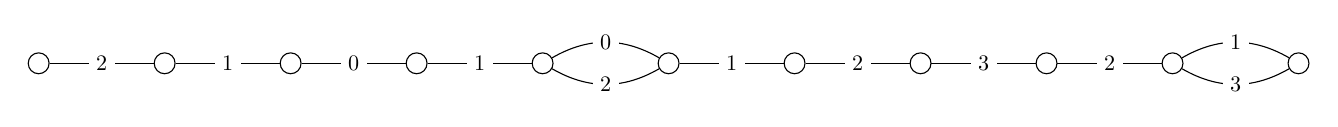
\begin{tikzpicture}[scale=.8]

      \begin{scope}[every node/.style={circle,draw, transform shape}]
        \node (1)  at (4,0)  {};
        \node (2)  at (6,0)  {};
        \node (3)  at (8,0)  {};
        \node (4)  at (10,0)  {};
        \node (5)  at (12,0) {};
        \node (6)  at (14,0)  {};
        \node (7)  at (0,0) {};
        \node (8)  at (16,0)  {};
        \node (9)  at (20,0)  {};
        \node (10) at (18,0) {};
        \node (11) at (2,0) {};
      \end{scope}

      \begin{scope}[every node/.style={fill=white, transform shape}]

        \begin{scope}[every edge/.style={draw}]
          \path (1)  edge node {$0$} (2);
          \path (3)  edge[bend left=30] node {$0$} (4);
          \path (1)  edge node {$1$} (11);
          \path (2)  edge node {$1$} (3);
          \path (4)  edge node {$1$} (5);
          \path (9)  edge[bend right=30] node {$1$} (10);
          \path (3)  edge[bend right=30] node {$2$} (4);
          \path (5)  edge node {$2$} (6);
          \path (7)  edge node {$2$} (11);
          \path (8)  edge node {$2$} (10);
          \path (6)  edge node {$3$} (8);
          \path (9)  edge[bend left=30] node {$3$} (10);
        \end{scope}
      \end{scope}

    \end{tikzpicture}
    \caption{}
    \label{r4-1-13}
  \end{center}
\end{figure}

\begin{figure}[H]
  \begin{center}
    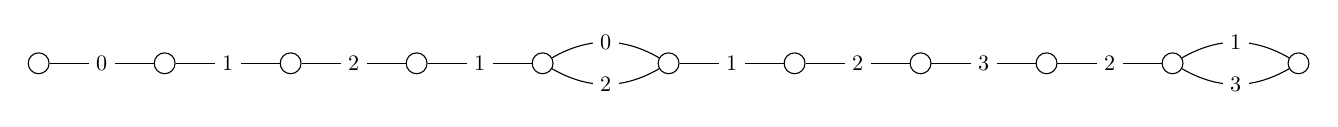
\begin{tikzpicture}[scale=.8]

      \begin{scope}[every node/.style={circle,draw, transform shape}]
        \node (1)  at (20,0) {};
        \node (2)  at (18,0) {};
        \node (3)  at (16,0) {};
        \node (4)  at (14,0)  {};
        \node (5)  at (12,0)  {};
        \node (6)  at (10,0)  {};
        \node (7)  at (8,0)  {};
        \node (8)  at (6,0)  {};
        \node (9)  at (4,0)  {};
        \node (10) at (2,0)  {};
        \node (11) at (0,0)  {};
      \end{scope}

      \begin{scope}[every node/.style={fill=white, transform shape}]

        \begin{scope}[every edge/.style={draw}]
          \path (1)  edge[bend left=30] node {$3$} (2);
          \path (3)  edge node {$3$} (4);
          \path (2)  edge node {$2$} (3);
          \path (4)  edge node {$2$} (5);
          \path (6)  edge[bend left=30] node {$2$} (7);
          \path (8)  edge node {$2$} (9);
          \path (1)  edge[bend right=30] node {$1$} (2);
          \path (5)  edge node {$1$} (6);
          \path (7)  edge node {$1$} (8);
          \path (9)  edge node {$1$} (10);
          \path (6)  edge[bend right=30] node {$0$} (7);
          \path (10) edge node {$0$} (11);
        \end{scope}
      \end{scope}

    \end{tikzpicture}
    \caption{}
    \label{r4-1-14}
  \end{center}
\end{figure}

\subsubsection{Length 2}

\begin{figure}[H]
  \begin{center}
    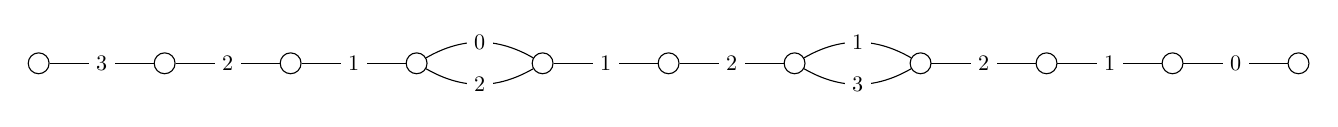
\begin{tikzpicture}[scale=.8]

      \begin{scope}[every node/.style={circle,draw, transform shape}]
        \node (1)  at (8,0) {};
        \node (2)  at (6,0)  {};
        \node (3)  at (18,0)  {};
        \node (4)  at (20,0)  {};
        \node (5)  at (0,0)  {};
        \node (6)  at (2,0)  {};
        \node (7)  at (4,0)  {};
        \node (8)  at (10,0)  {};
        \node (9)  at (12,0)  {};
        \node (10) at (14,0)  {};
        \node (11) at (16,0) {};
      \end{scope}

      \begin{scope}[every node/.style={fill=white, transform shape}]

        \begin{scope}[every edge/.style={draw}]
          \path (1)  edge[bend right=30] node {$0$} (2);
          \path (3)  edge node {$0$} (4);
          \path (1)  edge node {$1$} (8);
          \path (2)  edge node {$1$} (7);
          \path (3)  edge node {$1$} (11);
          \path (9)  edge[bend left=30] node {$1$} (10);
          \path (1)  edge[bend left=30] node {$2$} (2);
          \path (6)  edge node {$2$} (7);
          \path (8)  edge node {$2$} (9);
          \path (10) edge node {$2$} (11);
          \path (5)  edge node {$3$} (6);
          \path (9)  edge[bend right=30] node {$3$} (10);
        \end{scope}
      \end{scope}

    \end{tikzpicture}
    \caption{}
    \label{r4-1-15}
  \end{center}
\end{figure}

\begin{figure}[H]
  \begin{center}
    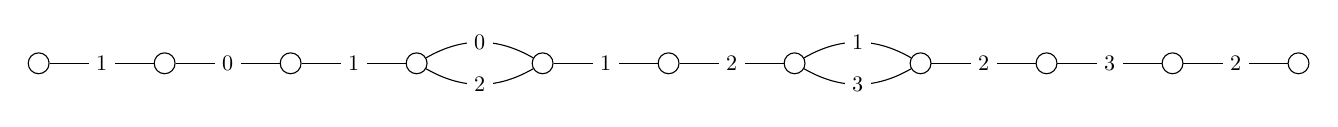
\begin{tikzpicture}[scale=.8]

      \begin{scope}[every node/.style={circle,draw, transform shape}]
        \node (1)  at (8,0)  {};
        \node (2)  at (6,0)  {};
        \node (3)  at (4,0)  {};
        \node (4)  at (2,0)  {};
        \node (5)  at (0,0) {};
        \node (6)  at (18,0)  {};
        \node (7)  at (20,0)  {};
        \node (8)  at (16,0)  {};
        \node (9)  at (14,0)  {};
        \node (10) at (12,0) {};
        \node (11) at (10,0) {};
      \end{scope}

      \begin{scope}[every node/.style={fill=white, transform shape}]

        \begin{scope}[every edge/.style={draw}]
          \path (1)  edge[bend right=30] node {$0$} (2);
          \path (3)  edge node {$0$} (4);
          \path (1)  edge node {$1$} (11);
          \path (2)  edge node {$1$} (3);
          \path (4)  edge node {$1$} (5);
          \path (9)  edge[bend right=30] node {$1$} (10);
          \path (1)  edge[bend left=30] node {$2$} (2);
          \path (6)  edge node {$2$} (7);
          \path (8)  edge node {$2$} (9);
          \path (10) edge node {$2$} (11);
          \path (6)  edge node {$3$} (8);
          \path (9)  edge[bend left=30] node {$3$} (10);
        \end{scope}
      \end{scope}

    \end{tikzpicture}
    \caption{}
    \label{r4-1-16}
  \end{center}
\end{figure}

\begin{figure}[H]
  \begin{center}
    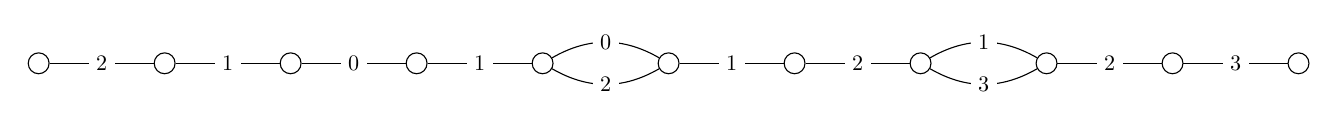
\begin{tikzpicture}[scale=.8]

      \begin{scope}[every node/.style={circle,draw, transform shape}]
        \node (1)  at (10,0)  {};
        \node (2)  at (8,0)  {};
        \node (3)  at (6,0)  {};
        \node (4)  at (4,0)  {};
        \node (5)  at (2,0) {};
        \node (6)  at (0,0) {};
        \node (7)  at (20,0) {};
        \node (8)  at (18,0)  {};
        \node (9)  at (16,0)  {};
        \node (10) at (14,0) {};
        \node (11) at (12,0) {};
      \end{scope}

      \begin{scope}[every node/.style={fill=white, transform shape}]

        \begin{scope}[every edge/.style={draw}]
          \path (1)  edge[bend right=30] node {$0$} (2);
          \path (3)  edge node {$0$} (4);
          \path (1)  edge node {$1$} (11);
          \path (2)  edge node {$1$} (3);
          \path (4)  edge node {$1$} (5);
          \path (9)  edge[bend right=30] node {$1$} (10);
          \path (1)  edge[bend left=30] node {$2$} (2);
          \path (5)  edge node {$2$} (6);
          \path (8)  edge node {$2$} (9);
          \path (10) edge node {$2$} (11);
          \path (7)  edge node {$3$} (8);
          \path (9)  edge[bend left=30] node {$3$} (10);
        \end{scope}
      \end{scope}

    \end{tikzpicture}
    \caption{}
    \label{r4-1-17}
  \end{center}
\end{figure}

\begin{figure}[H]
  \begin{center}
    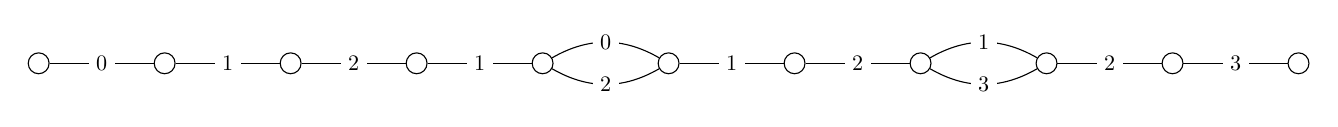
\begin{tikzpicture}[scale=.8]

      \begin{scope}[every node/.style={circle,draw, transform shape}]
        \node (1)  at (20,0) {};
        \node (2)  at (18,0) {};
        \node (3)  at (16,0) {};
        \node (4)  at (14,0)  {};
        \node (5)  at (12,0)  {};
        \node (6)  at (10,0)  {};
        \node (7)  at (8,0)  {};
        \node (8)  at (6,0)  {};
        \node (9)  at (4,0)  {};
        \node (10) at (2,0)  {};
        \node (11) at (0,0)  {};
      \end{scope}

      \begin{scope}[every node/.style={fill=white, transform shape}]

        \begin{scope}[every edge/.style={draw}]
          \path (1)  edge node {$3$} (2);
          \path (3)  edge[bend left=30] node {$3$} (4);
          \path (2)  edge node {$2$} (3);
          \path (4)  edge node {$2$} (5);
          \path (6)  edge[bend left=30] node {$2$} (7);
          \path (8)  edge node {$2$} (9);
          \path (3)  edge[bend right=30] node {$1$} (4);
          \path (5)  edge node {$1$} (6);
          \path (7)  edge node {$1$} (8);
          \path (9)  edge node {$1$} (10);
          \path (6)  edge[bend right=30] node {$0$} (7);
          \path (10) edge node {$0$} (11);
        \end{scope}
      \end{scope}

    \end{tikzpicture}
    \caption{}
    \label{r4-1-18}
  \end{center}
\end{figure}

\begin{figure}[H]
  \begin{center}
    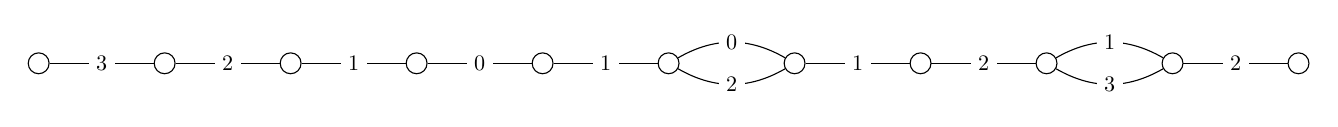
\begin{tikzpicture}[scale=.8]

      \begin{scope}[every node/.style={circle,draw, transform shape}]
        \node (1)  at (12,0)  {};
        \node (2)  at (10,0)  {};
        \node (3)  at (8,0)  {};
        \node (4)  at (6,0)  {};
        \node (5)  at (4,0) {};
        \node (6)  at (2,0) {};
        \node (7)  at (0,0) {};
        \node (8)  at (20,0)  {};
        \node (9)  at (18,0)  {};
        \node (10) at (16,0) {};
        \node (11) at (14,0) {};
      \end{scope}

      \begin{scope}[every node/.style={fill=white, transform shape}]

        \begin{scope}[every edge/.style={draw}]
          \path (1)  edge[bend right=30] node {$0$} (2);
          \path (3)  edge node {$0$} (4);
          \path (1)  edge node {$1$} (11);
          \path (2)  edge node {$1$} (3);
          \path (4)  edge node {$1$} (5);
          \path (9)  edge[bend right=30] node {$1$} (10);
          \path (1)  edge[bend left=30] node {$2$} (2);
          \path (5)  edge node {$2$} (6);
          \path (8)  edge node {$2$} (9);
          \path (10) edge node {$2$} (11);
          \path (6)  edge node {$3$} (7);
          \path (9)  edge[bend left=30] node {$3$} (10);
        \end{scope}
      \end{scope}

    \end{tikzpicture}
    \caption{}
    \label{r4-1-19}
  \end{center}
\end{figure}

\begin{figure}[H]
  \begin{center}
    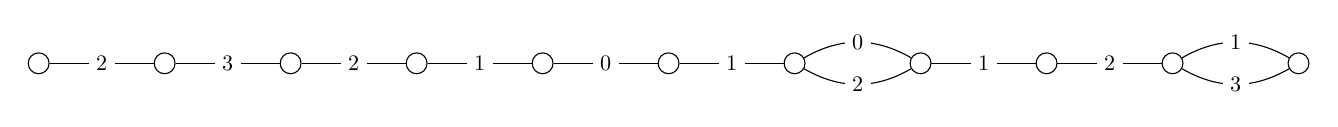
\begin{tikzpicture}[scale=.8]

      \begin{scope}[every node/.style={circle,draw, transform shape}]
        \node (1)  at (14,0)  {};
        \node (2)  at (12,0)  {};
        \node (3)  at (10,0)  {};
        \node (4)  at (8,0)  {};
        \node (5)  at (6,0) {};
        \node (6)  at (4,0)  {};
        \node (7)  at (2,0) {};
        \node (8)  at (0,0)  {};
        \node (9)  at (20,0)  {};
        \node (10) at (18,0) {};
        \node (11) at (16,0) {};
      \end{scope}

      \begin{scope}[every node/.style={fill=white, transform shape}]

        \begin{scope}[every edge/.style={draw}]
          \path (1)  edge[bend right=30] node {$0$} (2);
          \path (3)  edge node {$0$} (4);
          \path (1)  edge node {$1$} (11);
          \path (2)  edge node {$1$} (3);
          \path (4)  edge node {$1$} (5);
          \path (9)  edge[bend right=30] node {$1$} (10);
          \path (1)  edge[bend left=30] node {$2$} (2);
          \path (5)  edge node {$2$} (6);
          \path (7)  edge node {$2$} (8);
          \path (10) edge node {$2$} (11);
          \path (6)  edge node {$3$} (7);
          \path (9)  edge[bend left=30] node {$3$} (10);
        \end{scope}
      \end{scope}

    \end{tikzpicture}
    \caption{}
    \label{r4-1-20}
  \end{center}
\end{figure}

\begin{figure}[H]
  \begin{center}

    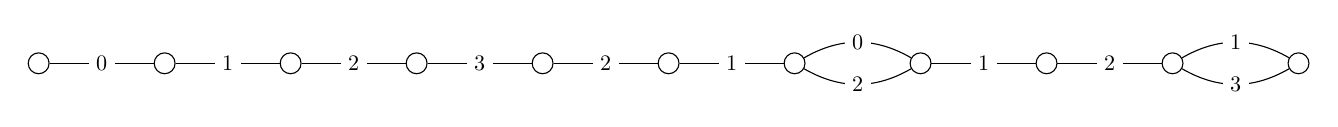
\begin{tikzpicture}[scale=.8]

      \begin{scope}[every node/.style={circle,draw, transform shape}]
        \node (1)  at (8,0) {};
        \node (2)  at (6,0)  {};
        \node (3)  at (18,0)  {};
        \node (4)  at (20,0)  {};
        \node (5)  at (0,0)  {};
        \node (6)  at (2,0)  {};
        \node (7)  at (4,0)  {};
        \node (8)  at (10,0)  {};
        \node (9)  at (12,0)  {};
        \node (10) at (14,0)  {};
        \node (11) at (16,0) {};
      \end{scope}

      \begin{scope}[every node/.style={fill=white, transform shape}]

        \begin{scope}[every edge/.style={draw}]
          \path (1)  edge node {$3$} (2);
          \path (3)  edge[bend right=30] node {$3$} (4);
          \path (1)  edge node {$2$} (8);
          \path (2)  edge node {$2$} (7);
          \path (3)  edge node {$2$} (11);
          \path (9)  edge[bend right=30] node {$2$} (10);
          \path (3)  edge[bend left=30] node {$1$} (4);
          \path (6)  edge node {$1$} (7);
          \path (8)  edge node {$1$} (9);
          \path (10) edge node {$1$} (11);
          \path (5)  edge node {$0$} (6);
          \path (9)  edge[bend left=30] node {$0$} (10);
        \end{scope}
      \end{scope}

    \end{tikzpicture}
    \caption{}
    \label{r4-1-21}
  \end{center}
\end{figure}

\subsection{One double edge and one alternating square}
\label{rank4-2-2-4transpositions}


\subsubsection{Length 4}

\begin{figure}[H]
  \begin{center}
    \begin{tikzpicture}[scale=.8]

      \begin{scope}[every node/.style={circle,draw, transform shape}]
        \node (1)  at (0,2) {};
        \node (2)  at (2,2) {};
        \node (3)  at (4,2) {};
        \node (4)  at (6,2)  {};
        \node (5)  at (8,2)  {};
        \node (6)  at (10,2)  {};
        \node (7)  at (12,2)  {};
        \node (8)  at (10,0)  {};
        \node (9)  at (12,0)  {};
        \node (10) at (14,0)  {};
        \node (11) at (14,2)  {};
      \end{scope}

      \begin{scope}[every node/.style={fill=white, transform shape}]

        \begin{scope}[every edge/.style={draw}]
          \path (1)  edge[bend left=30] node {$0$} (2);
          \path (3)  edge node {$0$} (4);
          \path (2)  edge node {$1$} (3);
          \path (4)  edge node {$1$} (5);
          \path (6)  edge node {$1$} (7);
          \path (8)  edge node {$1$} (9);
          \path (1)  edge[bend right=30] node {$2$} (2);
          \path (5)  edge node {$2$} (6);
          \path (7)  edge node {$2$} (11);
          \path (9)  edge node {$2$} (10);
          \path (6)  edge node {$3$} (8);
          \path (7)  edge node {$3$} (9);
        \end{scope}
      \end{scope}

    \end{tikzpicture}
    \caption{}
    \label{r4-2-1}
  \end{center}
\end{figure}

\begin{figure}[H]
  \begin{center}
    \begin{tikzpicture}[scale=.8]

      \begin{scope}[every node/.style={circle,draw, transform shape}]
        \node (1)  at (0,2) {};
        \node (2)  at (2,2) {};
        \node (3)  at (4,2) {};
        \node (4)  at (6,2)  {};
        \node (5)  at (8,2)  {};
        \node (6)  at (10,2)  {};
        \node (7)  at (12,2)  {};
        \node (8)  at (12,0)  {};
        \node (9)  at (10,0)  {};
        \node (10) at (8,0)  {};
        \node (11) at (14,0)  {};
      \end{scope}

      \begin{scope}[every node/.style={fill=white, transform shape}]

        \begin{scope}[every edge/.style={draw}]
          \path (1)  edge[bend left=30] node {$0$} (2);
          \path (3)  edge node {$0$} (4);
          \path (2)  edge node {$1$} (3);
          \path (4)  edge node {$1$} (5);
          \path (6)  edge node {$1$} (7);
          \path (8)  edge node {$1$} (9);
          \path (1)  edge[bend right=30] node {$2$} (2);
          \path (5)  edge node {$2$} (6);
          \path (8)  edge node {$2$} (11);
          \path (9)  edge node {$2$} (10);
          \path (6)  edge node {$3$} (9);
          \path (7)  edge node {$3$} (8);
        \end{scope}
      \end{scope}

    \end{tikzpicture}
    \caption{}
    \label{r4-2-2}
  \end{center}
\end{figure}

\begin{figure}[H]
  \begin{center}
    \begin{tikzpicture}[scale=.8]

      \begin{scope}[every node/.style={circle,draw, transform shape}]
        \node (1)  at (0,2) {};
        \node (2)  at (2,2) {};
        \node (3)  at (4,2) {};
        \node (4)  at (6,2)  {};
        \node (5)  at (8,2)  {};
        \node (6)  at (10,2)  {};
        \node (7)  at (12,2)  {};
        \node (8)  at (10,0)  {};
        \node (9)  at (12,0)  {};
        \node (10) at (8,0)  {};
        \node (11) at (14,2)  {};
      \end{scope}

      \begin{scope}[every node/.style={fill=white, transform shape}]

        \begin{scope}[every edge/.style={draw}]
          \path (1)  edge[bend left=30] node {$0$} (2);
          \path (3)  edge node {$0$} (4);
          \path (2)  edge node {$1$} (3);
          \path (4)  edge node {$1$} (5);
          \path (6)  edge node {$1$} (7);
          \path (8)  edge node {$1$} (9);
          \path (1)  edge[bend right=30] node {$2$} (2);
          \path (5)  edge node {$2$} (6);
          \path (7)  edge node {$2$} (11);
          \path (8)  edge node {$2$} (10);
          \path (6)  edge node {$3$} (8);
          \path (7)  edge node {$3$} (9);
        \end{scope}
      \end{scope}

    \end{tikzpicture}
    \caption{}
    \label{r4-2-3}
  \end{center}
\end{figure}

\subsubsection{Length 2}

\begin{figure}[H]
  \begin{center}
    \begin{tikzpicture}[scale=.8]

      \begin{scope}[every node/.style={circle,draw, transform shape}]
        \node (1)  at (0,2) {};
        \node (2)  at (2,2) {};
        \node (3)  at (4,2) {};
        \node (4)  at (6,2)  {};
        \node (5)  at (8,2)  {};
        \node (6)  at (10,2)  {};
        \node (7)  at (12,2)  {};
        \node (8)  at (10,0)  {};
        \node (9)  at (12,0)  {};
        \node (10) at (14,0)  {};
        \node (11) at (14,2)  {};
      \end{scope}

      \begin{scope}[every node/.style={fill=white, transform shape}]

        \begin{scope}[every edge/.style={draw}]
          \path (1)  edge node {$0$} (2);
          \path (3)  edge[bend left=30] node {$0$} (4);
          \path (2)  edge node {$1$} (3);
          \path (4)  edge node {$1$} (5);
          \path (6)  edge node {$1$} (7);
          \path (8)  edge node {$1$} (9);
          \path (3)  edge[bend right=30] node {$2$} (4);
          \path (5)  edge node {$2$} (6);
          \path (7)  edge node {$2$} (11);
          \path (9)  edge node {$2$} (10);
          \path (6)  edge node {$3$} (8);
          \path (7)  edge node {$3$} (9);
        \end{scope}
      \end{scope}

    \end{tikzpicture}
    \caption{}
    \label{r4-2-4}
  \end{center}
\end{figure}

\begin{figure}[H]
  \begin{center}
    \begin{tikzpicture}[scale=.8]

      \begin{scope}[every node/.style={circle,draw, transform shape}]
        \node (1)  at (0,2)  {};
        \node (2)  at (2,2)  {};
        \node (3)  at (4,2)  {};
        \node (4)  at (6,2)  {};
        \node (5)  at (8,2) {};
        \node (6)  at (10,2)  {};
        \node (7)  at (12,2) {};
        \node (8)  at (12,0)  {};
        \node (9)  at (10,0)  {};
        \node (10) at (8,0) {};
        \node (11) at (14,0) {};
      \end{scope}

      \begin{scope}[every node/.style={fill=white, transform shape}]

        \begin{scope}[every edge/.style={draw}]
          \path (1)  edge node {$0$} (2);
          \path (3)  edge[bend left=30] node {$0$} (4);
          \path (2)  edge node {$1$} (3);
          \path (4)  edge node {$1$} (5);
          \path (6)  edge node {$1$} (7);
          \path (8)  edge node {$1$} (9);
          \path (3)  edge[bend right=30] node {$2$} (4);
          \path (5)  edge node {$2$} (6);
          \path (8)  edge node {$2$} (11);
          \path (9)  edge node {$2$} (10);
          \path (6)  edge node {$3$} (9);
          \path (7)  edge node {$3$} (8);
        \end{scope}
      \end{scope}

    \end{tikzpicture}
    \caption{}
    \label{r4-2-5}
  \end{center}
\end{figure}

\begin{figure}[H]
  \begin{center}
    \begin{tikzpicture}[scale=.8]

      \begin{scope}[every node/.style={circle,draw, transform shape}]
        \node (1)  at (0,2) {};
        \node (2)  at (2,2) {};
        \node (3)  at (4,2) {};
        \node (4)  at (6,2)  {};
        \node (5)  at (8,2)  {};
        \node (6)  at (10,2)  {};
        \node (7)  at (12,2)  {};
        \node (8)  at (10,0)  {};
        \node (9)  at (12,0)  {};
        \node (10) at (8,0)  {};
        \node (11) at (14,2)  {};
      \end{scope}

      \begin{scope}[every node/.style={fill=white, transform shape}]

        \begin{scope}[every edge/.style={draw}]
          \path (1)  edge node {$0$} (2);
          \path (3)  edge[bend left=30] node {$0$} (4);
          \path (2)  edge node {$1$} (3);
          \path (4)  edge node {$1$} (5);
          \path (6)  edge node {$1$} (7);
          \path (8)  edge node {$1$} (9);
          \path (3)  edge[bend right=30] node {$2$} (4);
          \path (5)  edge node {$2$} (6);
          \path (7)  edge node {$2$} (11);
          \path (8)  edge node {$2$} (10);
          \path (6)  edge node {$3$} (8);
          \path (7)  edge node {$3$} (9);
        \end{scope}
      \end{scope}

    \end{tikzpicture}
    \caption{}
    \label{r4-2-6}
  \end{center}
\end{figure}

\begin{figure}[H]
  \begin{center}
    \begin{tikzpicture}[scale=.8]

      \begin{scope}[every node/.style={circle,draw, transform shape}]
        \node (1)  at (12,2) {};
        \node (2)  at (10,2)  {};
        \node (3)  at (0,2)  {};
        \node (4)  at (-2,2)  {};
        \node (5)  at (2,2)  {};
        \node (6)  at (8,2)  {};
        \node (7)  at (6,2)  {};
        \node (8)  at (4,2)  {};
        \node (9)  at (4,0)  {};
        \node (10) at (6,0)  {};
        \node (11) at (2,0) {};
      \end{scope}

      \begin{scope}[every node/.style={fill=white, transform shape}]

        \begin{scope}[every edge/.style={draw}]
          \path (1)  edge node {$0$} (2);
          \path (3)  edge[bend right=30] node {$0$} (4);
          \path (2)  edge node {$1$} (6);
          \path (3)  edge node {$1$} (5);
          \path (7)  edge node {$1$} (8);
          \path (9)  edge node {$1$} (10);
          \path (3)  edge[bend left=30] node {$2$} (4);
          \path (5)  edge node {$2$} (8);
          \path (6)  edge node {$2$} (7);
          \path (9)  edge node {$2$} (11);
          \path (7)  edge node {$3$} (10);
          \path (8)  edge node {$3$} (9);
        \end{scope}
      \end{scope}

    \end{tikzpicture}
    \caption{}
    \label{r4-2-7}
  \end{center}
\end{figure}

\begin{figure}[H]
  \begin{center}
    \begin{tikzpicture}[scale=.8]

      \begin{scope}[every node/.style={circle,draw, transform shape}]
        \node (1)  at (12,2) {};
        \node (2)  at (10,2)  {};
        \node (3)  at (0,2)  {};
        \node (4)  at (-2,2)  {};
        \node (5)  at (2,2)  {};
        \node (6)  at (8,2)  {};
        \node (7)  at (6,2)  {};
        \node (8)  at (4,2)  {};
        \node (9)  at (6,0)  {};
        \node (10) at (4,0)  {};
        \node (11) at (8,0) {};
      \end{scope}

      \begin{scope}[every node/.style={fill=white, transform shape}]

        \begin{scope}[every edge/.style={draw}]
          \path (1)  edge node {$0$} (2);
          \path (3)  edge[bend right=30] node {$0$} (4);
          \path (2)  edge node {$1$} (6);
          \path (3)  edge node {$1$} (5);
          \path (7)  edge node {$1$} (8);
          \path (9)  edge node {$1$} (10);
          \path (3)  edge[bend left=30] node {$2$} (4);
          \path (5)  edge node {$2$} (8);
          \path (6)  edge node {$2$} (7);
          \path (9)  edge node {$2$} (11);
          \path (7)  edge node {$3$} (9);
          \path (8)  edge node {$3$} (10);
        \end{scope}
      \end{scope}

    \end{tikzpicture}
    \caption{}
    \label{r4-2-8}
  \end{center}
\end{figure}

\begin{figure}[H]
  \begin{center}
    \begin{tikzpicture}[scale=.8]

      \begin{scope}[every node/.style={circle,draw, transform shape}]
        \node (1)  at (14,2) {};
        \node (2)  at (12,2)  {};
        \node (3)  at (2,2)  {};
        \node (4)  at (0,2)  {};
        \node (5)  at (4,2)  {};
        \node (6)  at (10,2)  {};
        \node (7)  at (6,0)  {};
        \node (8)  at (6,2)  {};
        \node (9)  at (8,2)  {};
        \node (10) at (8,0)  {};
        \node (11) at (10,0) {};
      \end{scope}

      \begin{scope}[every node/.style={fill=white, transform shape}]

        \begin{scope}[every edge/.style={draw}]
          \path (1)  edge node {$0$} (2);
          \path (3)  edge[bend right=30] node {$0$} (4);
          \path (2)  edge node {$1$} (6);
          \path (3)  edge node {$1$} (5);
          \path (7)  edge node {$1$} (8);
          \path (9)  edge node {$1$} (10);
          \path (3)  edge[bend left=30] node {$2$} (4);
          \path (5)  edge node {$2$} (8);
          \path (6)  edge node {$2$} (9);
          \path (10) edge node {$2$} (11);
          \path (7)  edge node {$3$} (10);
          \path (8)  edge node {$3$} (9);
        \end{scope}
      \end{scope}

    \end{tikzpicture}
    \caption{}
    \label{r4-2-9}
  \end{center}
\end{figure}

\begin{figure}[H]
  \begin{center}
    \begin{tikzpicture}[scale=.8]

      \begin{scope}[every node/.style={circle,draw, transform shape}]
        \node (1)  at (14,2) {};
        \node (2)  at (12,2)  {};
        \node (3)  at (2,2)  {};
        \node (4)  at (0,2)  {};
        \node (5)  at (4,2)  {};
        \node (6)  at (10,2)  {};
        \node (7)  at (8,0)  {};
        \node (8)  at (8,2)  {};
        \node (9)  at (6,2)  {};
        \node (10) at (6,0)  {};
        \node (11) at (4,0) {};
      \end{scope}

      \begin{scope}[every node/.style={fill=white, transform shape}]

        \begin{scope}[every edge/.style={draw}]
          \path (1)  edge node {$0$} (2);
          \path (3)  edge[bend right=30] node {$0$} (4);
          \path (2)  edge node {$1$} (6);
          \path (3)  edge node {$1$} (5);
          \path (7)  edge node {$1$} (8);
          \path (9)  edge node {$1$} (10);
          \path (3)  edge[bend left=30] node {$2$} (4);
          \path (5)  edge node {$2$} (9);
          \path (6)  edge node {$2$} (8);
          \path (10) edge node {$2$} (11);
          \path (7)  edge node {$3$} (10);
          \path (8)  edge node {$3$} (9);
        \end{scope}
      \end{scope}

    \end{tikzpicture}
    \caption{}
    \label{r4-2-10}
  \end{center}
\end{figure}

\begin{figure}[H]
  \begin{center}
    \begin{tikzpicture}[scale=.8]

      \begin{scope}[every node/.style={circle,draw, transform shape}]
        \node (1)  at (14,0) {};
        \node (2)  at (12,0)  {};
        \node (3)  at (2,2)  {};
        \node (4)  at (0,2)  {};
        \node (5)  at (4,2)  {};
        \node (6)  at (10,0)  {};
        \node (7)  at (6,0)  {};
        \node (8)  at (8,0)  {};
        \node (9)  at (6,2)  {};
        \node (10) at (8,2)  {};
        \node (11) at (10,2) {};
      \end{scope}

      \begin{scope}[every node/.style={fill=white, transform shape}]

        \begin{scope}[every edge/.style={draw}]
          \path (1)  edge node {$0$} (2);
          \path (3)  edge[bend right=30] node {$0$} (4);
          \path (2)  edge node {$1$} (6);
          \path (3)  edge node {$1$} (5);
          \path (7)  edge node {$1$} (8);
          \path (9)  edge node {$1$} (10);
          \path (3)  edge[bend left=30] node {$2$} (4);
          \path (5)  edge node {$2$} (9);
          \path (6)  edge node {$2$} (8);
          \path (10) edge node {$2$} (11);
          \path (7)  edge node {$3$} (9);
          \path (8)  edge node {$3$} (10);
        \end{scope}
      \end{scope}

    \end{tikzpicture}
    \caption{}
    \label{r4-2-11}
  \end{center}
\end{figure}

\begin{figure}[H]
  \begin{center}
    \begin{tikzpicture}[scale=.8]

      \begin{scope}[every node/.style={circle,draw, transform shape}]
        \node (1)  at (14,0) {};
        \node (2)  at (12,0)  {};
        \node (3)  at (2,2)  {};
        \node (4)  at (0,2)  {};
        \node (5)  at (4,2)  {};
        \node (6)  at (10,0)  {};
        \node (7)  at (8,2)  {};
        \node (8)  at (6,2)  {};
        \node (9)  at (8,0)  {};
        \node (10) at (6,0)  {};
        \node (11) at (4,0) {};
      \end{scope}

      \begin{scope}[every node/.style={fill=white, transform shape}]

        \begin{scope}[every edge/.style={draw}]
          \path (1)  edge node {$0$} (2);
          \path (3)  edge[bend right=30] node {$0$} (4);
          \path (2)  edge node {$1$} (6);
          \path (3)  edge node {$1$} (5);
          \path (7)  edge node {$1$} (8);
          \path (9)  edge node {$1$} (10);
          \path (3)  edge[bend left=30] node {$2$} (4);
          \path (5)  edge node {$2$} (8);
          \path (6)  edge node {$2$} (9);
          \path (10) edge node {$2$} (11);
          \path (7)  edge node {$3$} (9);
          \path (8)  edge node {$3$} (10);
        \end{scope}
      \end{scope}

    \end{tikzpicture}
    \caption{}
    \label{r4-2-12}
  \end{center}
\end{figure}

\subsection{Two alternating squares}
\label{rank4-2-3-4transpositions}

\subsubsection{Length 4}

\begin{figure}[H]
  \begin{center}
    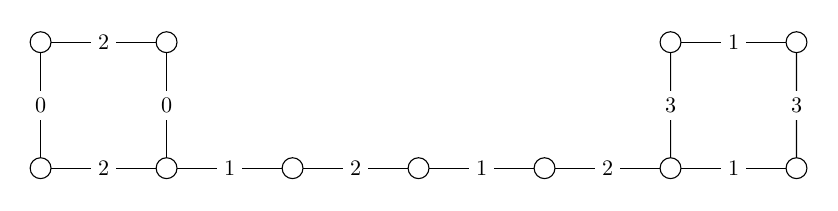
\begin{tikzpicture}[scale=.8]

      \begin{scope}[every node/.style={circle,draw, transform shape}]
        \node (1)  at (2,2)  {};
        \node (2)  at (2,0)  {};
        \node (3)  at (0,0)  {};
        \node (4)  at (0,2)  {};
        \node (5)  at (4,0)  {};
        \node (6)  at (6,0)  {};
        \node (7)  at (8,0)  {};
        \node (8)  at (10,0)  {};
        \node (9)  at (12,0)  {};
        \node (10) at (12,2) {};
        \node (11) at (10,2) {};
      \end{scope}

      \begin{scope}[every node/.style={fill=white, transform shape}]

        \begin{scope}[every edge/.style={draw}]
          \path (1)  edge node {$0$} (2);
          \path (3)  edge node {$0$} (4);
          \path (2)  edge node {$1$} (5);
          \path (6)  edge node {$1$} (7);
          \path (8)  edge node {$1$} (9);
          \path (10) edge node {$1$} (11);
          \path (1)  edge node {$2$} (4);
          \path (2)  edge node {$2$} (3);
          \path (5)  edge node {$2$} (6);
          \path (7)  edge node {$2$} (8);
          \path (8)  edge node {$3$} (11);
          \path (9)  edge node {$3$} (10);
        \end{scope}
      \end{scope}

    \end{tikzpicture}
    \caption{}
    \label{r4-3-1}
  \end{center}
\end{figure}

\subsubsection{Length 2}

\begin{figure}[H]
  \begin{center}
    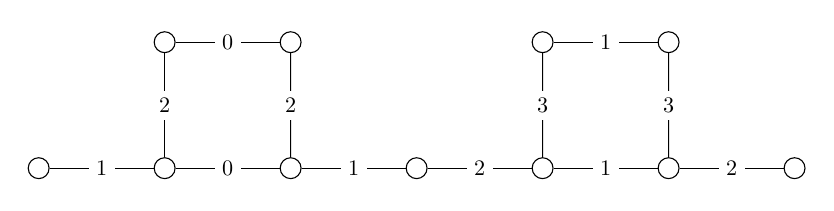
\begin{tikzpicture}[scale=.8]

      \begin{scope}[every node/.style={circle,draw, transform shape}]
        \node (1)  at (4,0)  {};
        \node (2)  at (2,0)  {};
        \node (3)  at (2,2)  {};
        \node (4)  at (4,2)  {};
        \node (5)  at (0,0)  {};
        \node (6)  at (6,0)  {};
        \node (7)  at (8,2)  {};
        \node (8)  at (10,2) {};
        \node (9)  at (8,0)  {};
        \node (10) at (10,0) {};
        \node (11) at (12,0) {};
      \end{scope}

      \begin{scope}[every node/.style={fill=white, transform shape}]

        \begin{scope}[every edge/.style={draw}]
          \path (1)  edge node {$0$} (2);
          \path (3)  edge node {$0$} (4);
          \path (1)  edge node {$1$} (6);
          \path (2)  edge node {$1$} (5);
          \path (7)  edge node {$1$} (8);
          \path (9)  edge node {$1$} (10);
          \path (1)  edge node {$2$} (4);
          \path (2)  edge node {$2$} (3);
          \path (6)  edge node {$2$} (9);
          \path (10) edge node {$2$} (11);
          \path (7)  edge node {$3$} (9);
          \path (8)  edge node {$3$} (10);
        \end{scope}
      \end{scope}

    \end{tikzpicture}
    \caption{}
    \label{r4-3-2}
  \end{center}
\end{figure}

\begin{figure}[H]
  \begin{center}
    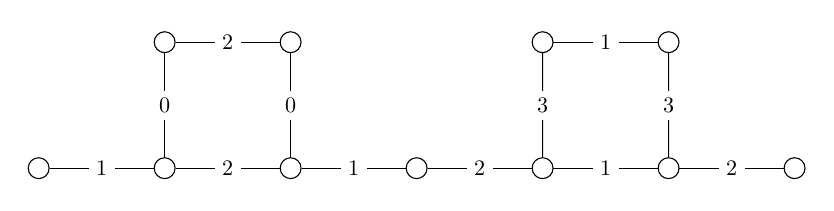
\begin{tikzpicture}[scale=.8]

      \begin{scope}[every node/.style={circle,draw, transform shape}]
        \node (1)  at (0,2) {};
        \node (2)  at (0,0)  {};
        \node (3)  at (-2,0)  {};
        \node (4)  at (-2,2)  {};
        \node (5)  at (-4,0)  {};
        \node (6)  at (2,0)  {};
        \node (7)  at (6,2)  {};
        \node (8)  at (4,2)  {};
        \node (9)  at (4,0)  {};
        \node (10) at (6,0)  {};
        \node (11) at (8,0) {};
      \end{scope}

      \begin{scope}[every node/.style={fill=white, transform shape}]

        \begin{scope}[every edge/.style={draw}]
          \path (1)  edge node {$0$} (2);
          \path (3)  edge node {$0$} (4);
          \path (2)  edge node {$1$} (6);
          \path (3)  edge node {$1$} (5);
          \path (7)  edge node {$1$} (8);
          \path (9)  edge node {$1$} (10);
          \path (1)  edge node {$2$} (4);
          \path (2)  edge node {$2$} (3);
          \path (6)  edge node {$2$} (9);
          \path (10) edge node {$2$} (11);
          \path (7)  edge node {$3$} (10);
          \path (8)  edge node {$3$} (9);
        \end{scope}
      \end{scope}

    \end{tikzpicture}
    \caption{}
    \label{r4-3-3}
  \end{center}
\end{figure}

\begin{figure}[H]
  \begin{center}
    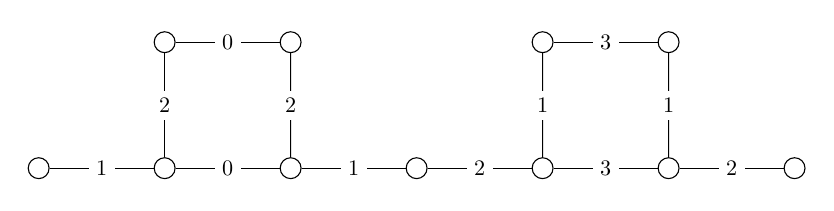
\begin{tikzpicture}[scale=.8]

      \begin{scope}[every node/.style={circle,draw, transform shape}]
        \node (1)  at (4,0)  {};
        \node (2)  at (2,0)  {};
        \node (3)  at (2,2)  {};
        \node (4)  at (4,2)  {};
        \node (5)  at (0,0)  {};
        \node (6)  at (6,0)  {};
        \node (7)  at (8,0)  {};
        \node (8)  at (8,2) {};
        \node (9)  at (10,2) {};
        \node (10) at (10,0) {};
        \node (11) at (12,0) {};
      \end{scope}

      \begin{scope}[every node/.style={fill=white, transform shape}]

        \begin{scope}[every edge/.style={draw}]
          \path (1)  edge node {$0$} (2);
          \path (3)  edge node {$0$} (4);
          \path (1)  edge node {$1$} (6);
          \path (2)  edge node {$1$} (5);
          \path (7)  edge node {$1$} (8);
          \path (9)  edge node {$1$} (10);
          \path (1)  edge node {$2$} (4);
          \path (2)  edge node {$2$} (3);
          \path (6)  edge node {$2$} (7);
          \path (10) edge node {$2$} (11);
          \path (7)  edge node {$3$} (10);
          \path (8)  edge node {$3$} (9);
        \end{scope}
      \end{scope}

    \end{tikzpicture}
    \caption{}
    \label{r4-3-4}
  \end{center}
\end{figure}

\begin{figure}[H]
  \begin{center}
    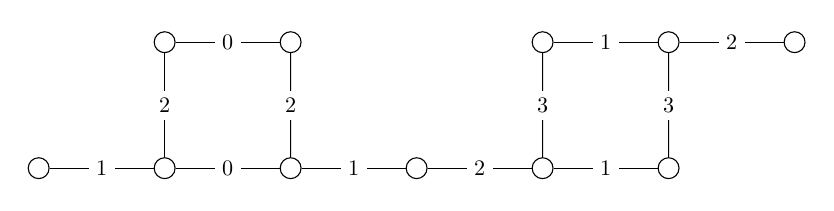
\begin{tikzpicture}[scale=.8]

      \begin{scope}[every node/.style={circle,draw, transform shape}]
        \node (1)  at (4,0)  {};
        \node (2)  at (2,0)  {};
        \node (3)  at (2,2)  {};
        \node (4)  at (4,2)  {};
        \node (5)  at (0,0)  {};
        \node (6)  at (6,0)  {};
        \node (7)  at (8,0)  {};
        \node (8)  at (10,0) {};
        \node (9)  at (8,2) {};
        \node (10) at (10,2) {};
        \node (11) at (12,2) {};
      \end{scope}

      \begin{scope}[every node/.style={fill=white, transform shape}]

        \begin{scope}[every edge/.style={draw}]
          \path (1)  edge node {$0$} (2);
          \path (3)  edge node {$0$} (4);
          \path (1)  edge node {$1$} (6);
          \path (2)  edge node {$1$} (5);
          \path (7)  edge node {$1$} (8);
          \path (9)  edge node {$1$} (10);
          \path (1)  edge node {$2$} (4);
          \path (2)  edge node {$2$} (3);
          \path (6)  edge node {$2$} (7);
          \path (10) edge node {$2$} (11);
          \path (7)  edge node {$3$} (9);
          \path (8)  edge node {$3$} (10);
        \end{scope}
      \end{scope}

    \end{tikzpicture}
    \caption{}
    \label{r4-3-5}
  \end{center}
\end{figure}

\begin{figure}[H]
  \begin{center}
    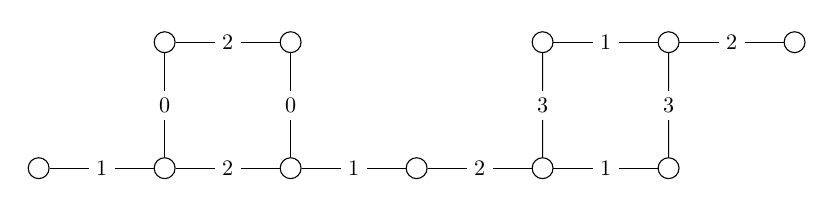
\begin{tikzpicture}[scale=.8]

      \begin{scope}[every node/.style={circle,draw, transform shape}]
        \node (1)  at (0,2) {};
        \node (2)  at (0,0)  {};
        \node (3)  at (-2,0)  {};
        \node (4)  at (-2,2)  {};
        \node (5)  at (-4,0)  {};
        \node (6)  at (2,0)  {};
        \node (7)  at (4,0)  {};
        \node (8)  at (6,0)  {};
        \node (9)  at (4,2)  {};
        \node (10) at (6,2)  {};
        \node (11) at (8,2) {};
      \end{scope}

      \begin{scope}[every node/.style={fill=white, transform shape}]

        \begin{scope}[every edge/.style={draw}]
          \path (1)  edge node {$0$} (2);
          \path (3)  edge node {$0$} (4);
          \path (2)  edge node {$1$} (6);
          \path (3)  edge node {$1$} (5);
          \path (7)  edge node {$1$} (8);
          \path (9)  edge node {$1$} (10);
          \path (1)  edge node {$2$} (4);
          \path (2)  edge node {$2$} (3);
          \path (6)  edge node {$2$} (7);
          \path (10) edge node {$2$} (11);
          \path (7)  edge node {$3$} (9);
          \path (8)  edge node {$3$} (10);
        \end{scope}
      \end{scope}

    \end{tikzpicture}
    \caption{}
    \label{r4-3-6}
  \end{center}
\end{figure}

\begin{figure}[H]
  \begin{center}
    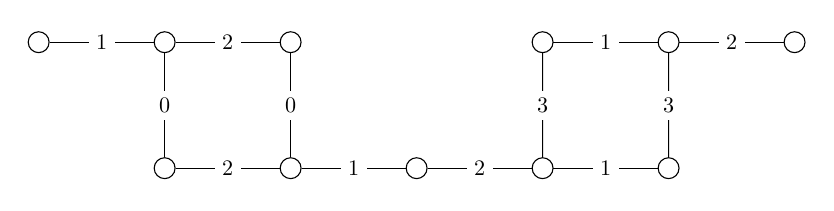
\begin{tikzpicture}[scale=.8]

      \begin{scope}[every node/.style={circle,draw, transform shape}]
        \node (1)  at (0,2) {};
        \node (2)  at (0,0)  {};
        \node (3)  at (-2,2)  {};
        \node (4)  at (-2,0)  {};
        \node (5)  at (-4,2)  {};
        \node (6)  at (2,0)  {};
        \node (7)  at (4,0)  {};
        \node (8)  at (6,0)  {};
        \node (9)  at (4,2)  {};
        \node (10) at (6,2)  {};
        \node (11) at (8,2) {};
      \end{scope}

      \begin{scope}[every node/.style={fill=white, transform shape}]

        \begin{scope}[every edge/.style={draw}]
          \path (1)  edge node {$0$} (2);
          \path (3)  edge node {$0$} (4);
          \path (2)  edge node {$1$} (6);
          \path (3)  edge node {$1$} (5);
          \path (7)  edge node {$1$} (8);
          \path (9)  edge node {$1$} (10);
          \path (1)  edge node {$2$} (3);
          \path (2)  edge node {$2$} (4);
          \path (6)  edge node {$2$} (7);
          \path (10) edge node {$2$} (11);
          \path (7)  edge node {$3$} (9);
          \path (8)  edge node {$3$} (10);
        \end{scope}
      \end{scope}

    \end{tikzpicture}
    \caption{}
    \label{r4-3-7}
  \end{center}
\end{figure}

\begin{figure}[H]
  \begin{center}
    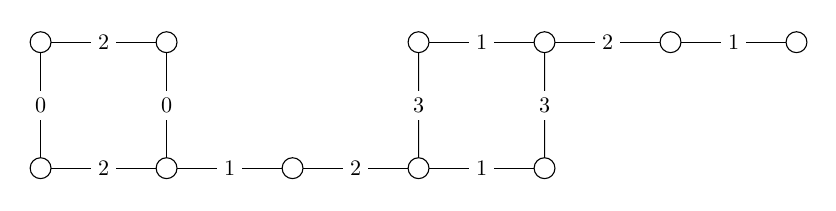
\begin{tikzpicture}[scale=.8]

      \begin{scope}[every node/.style={circle,draw, transform shape}]
        \node (1)  at (2,2)  {};
        \node (2)  at (2,0)  {};
        \node (3)  at (0,0)  {};
        \node (4)  at (0,2)  {};
        \node (5)  at (4,0)  {};
        \node (6)  at (6,0)  {};
        \node (7)  at (8,0)  {};
        \node (8)  at (8,2)  {};
        \node (9)  at (6,2)  {};
        \node (10) at (10,2)  {};
        \node (11) at (12,2) {};
      \end{scope}

      \begin{scope}[every node/.style={fill=white, transform shape}]

        \begin{scope}[every edge/.style={draw}]
          \path (1)  edge node {$0$} (2);
          \path (3)  edge node {$0$} (4);
          \path (2)  edge node {$1$} (5);
          \path (6)  edge node {$1$} (7);
          \path (8)  edge node {$1$} (9);
          \path (10) edge node {$1$} (11);
          \path (1)  edge node {$2$} (4);
          \path (2)  edge node {$2$} (3);
          \path (5)  edge node {$2$} (6);
          \path (8)  edge node {$2$} (10);
          \path (6)  edge node {$3$} (9);
          \path (7)  edge node {$3$} (8);
        \end{scope}
      \end{scope}

    \end{tikzpicture}
    \caption{}
    \label{r4-3-8}
  \end{center}
\end{figure}

\begin{figure}[H]
  \begin{center}
    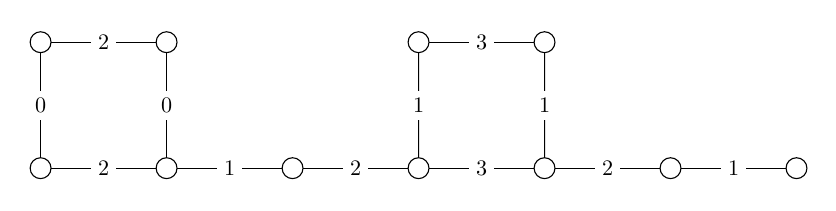
\begin{tikzpicture}[scale=.8]

      \begin{scope}[every node/.style={circle,draw, transform shape}]
        \node (1)  at (2,2)  {};
        \node (2)  at (2,0)  {};
        \node (3)  at (0,0)  {};
        \node (4)  at (0,2)  {};
        \node (5)  at (4,0)  {};
        \node (6)  at (6,0)  {};
        \node (7)  at (6,2)  {};
        \node (8)  at (8,0)  {};
        \node (9)  at (8,2)  {};
        \node (10) at (10,0)  {};
        \node (11) at (12,0) {};
      \end{scope}

      \begin{scope}[every node/.style={fill=white, transform shape}]

        \begin{scope}[every edge/.style={draw}]
          \path (1)  edge node {$0$} (2);
          \path (3)  edge node {$0$} (4);
          \path (2)  edge node {$1$} (5);
          \path (6)  edge node {$1$} (7);
          \path (8)  edge node {$1$} (9);
          \path (10) edge node {$1$} (11);
          \path (1)  edge node {$2$} (4);
          \path (2)  edge node {$2$} (3);
          \path (5)  edge node {$2$} (6);
          \path (8)  edge node {$2$} (10);
          \path (6)  edge node {$3$} (8);
          \path (7)  edge node {$3$} (9);
        \end{scope}
      \end{scope}

    \end{tikzpicture}
    \caption{}
    \label{r4-3-9}
  \end{center}
\end{figure}

\begin{figure}[H]
  \begin{center}
    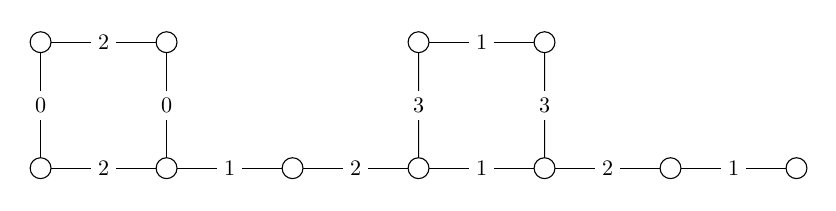
\begin{tikzpicture}[scale=.8]

      \begin{scope}[every node/.style={circle,draw, transform shape}]
        \node (1)  at (2,2)  {};
        \node (2)  at (2,0)  {};
        \node (3)  at (0,2)  {};
        \node (4)  at (0,0)  {};
        \node (5)  at (4,0)  {};
        \node (6)  at (6,0)  {};
        \node (7)  at (8,0)  {};
        \node (8)  at (10,0)  {};
        \node (9)  at (12,0)  {};
        \node (10) at (8,2) {};
        \node (11) at (6,2) {};
      \end{scope}

      \begin{scope}[every node/.style={fill=white, transform shape}]

        \begin{scope}[every edge/.style={draw}]
          \path (1)  edge node {$0$} (2);
          \path (3)  edge node {$0$} (4);
          \path (2)  edge node {$1$} (5);
          \path (6)  edge node {$1$} (7);
          \path (8)  edge node {$1$} (9);
          \path (10) edge node {$1$} (11);
          \path (1)  edge node {$2$} (3);
          \path (2)  edge node {$2$} (4);
          \path (5)  edge node {$2$} (6);
          \path (7)  edge node {$2$} (8);
          \path (6)  edge node {$3$} (11);
          \path (7)  edge node {$3$} (10);
        \end{scope}
      \end{scope}

    \end{tikzpicture}
    \caption{}
    \label{r4-3-10}
  \end{center}
\end{figure}


\section{Three 4-transpositions}
\label{rank4-3-4transpositions}

\subsection{Length 1}

\begin{figure}[H]
  \begin{center}
    \begin{tikzpicture}[scale=.8]

      \begin{scope}[every node/.style={circle,draw, transform shape}]
        \node (1)  at (2,2)  {};
        \node (2)  at (0,2)  {};
        \node (3)  at (14,0)  {};
        \node (4)  at (16,0) {};
        \node (5)  at (8,0)  {};
        \node (6)  at (10,0)  {};
        \node (7)  at (0,0)  {};
        \node (8)  at (2,0)  {};
        \node (9)  at (4,0)  {};
        \node (10) at (6,0)  {};
        \node (11) at (12,0)  {};
      \end{scope}

      \begin{scope}[every node/.style={fill=white, transform shape}]

        \begin{scope}[every edge/.style={draw}]
          \path (1)  edge[bend right=45] node {$0$} (2);
          \path (3)  edge node {$0$} (4);
          \path (1)  edge node {$1$} (8);
          \path (2)  edge node {$1$} (7);
          \path (3)  edge node {$1$} (11);
          \path (9)  edge[bend left=30] node {$1$} (10);
          \path (1)  edge node {$2$} (2);
          \path (5)  edge node {$2$} (10);
          \path (6)  edge node {$2$} (11);
          \path (8)  edge node {$2$} (9);
          \path (1)  edge[bend left=45] node {$3$} (2);
          \path (5)  edge node {$3$} (6);
          \path (7)  edge node {$3$} (8);
          \path (9)  edge[bend right=30] node {$3$} (10);
        \end{scope}
      \end{scope}

    \end{tikzpicture}
    \caption{}
    \label{r4-5-1}
  \end{center}
\end{figure}

\begin{figure}[H]
  \begin{center}
    \begin{tikzpicture}[scale=.8]

      \begin{scope}[every node/.style={circle,draw, transform shape}]
        \node (1)  at (4,2)  {};
        \node (2)  at (2,2)  {};
        \node (3)  at (12,0)  {};
        \node (4)  at (14,0) {};
        \node (5)  at (-2,0)  {};
        \node (6)  at (0,0)  {};
        \node (7)  at (2,0)  {};
        \node (8)  at (4,0)  {};
        \node (9)  at (6,0)  {};
        \node (10) at (8,0)  {};
        \node (11) at (10,0)  {};
      \end{scope}

      \begin{scope}[every node/.style={fill=white, transform shape}]

        \begin{scope}[every edge/.style={draw}]
          \path (1)  edge[bend right=45] node {$0$} (2);
          \path (3)  edge node {$0$} (4);
          \path (1)  edge node {$1$} (8);
          \path (2)  edge node {$1$} (7);
          \path (3)  edge node {$1$} (11);
          \path (9)  edge[bend left=30] node {$1$} (10);
          \path (1)  edge node {$2$} (2);
          \path (6)  edge node {$2$} (7);
          \path (8)  edge node {$2$} (9);
          \path (10) edge node {$2$} (11);
          \path (1)  edge[bend left=45] node {$3$} (2);
          \path (5)  edge node {$3$} (6);
          \path (7)  edge node {$3$} (8);
          \path (9)  edge[bend right=30] node {$3$} (10);
        \end{scope}
      \end{scope}

    \end{tikzpicture}
    \caption{}
    \label{r4-5-2}
  \end{center}
\end{figure}

\begin{figure}[H]
  \begin{center}
    \begin{tikzpicture}[scale=.8]

      \begin{scope}[every node/.style={circle,draw, transform shape}]
        \node (1)  at (-4,2)  {};
        \node (2)  at (-6,2)  {};
        \node (3)  at (-10,0)  {};
        \node (4)  at (-12,0) {};
        \node (5)  at (4,0)  {};
        \node (6)  at (2,0)  {};
        \node (7)  at (-6,0)  {};
        \node (8)  at (-4,0)  {};
        \node (9)  at (-2,0)  {};
        \node (10) at (0,0)  {};
        \node (11) at (-8,0)  {};
      \end{scope}

      \begin{scope}[every node/.style={fill=white, transform shape}]

        \begin{scope}[every edge/.style={draw}]
          \path (1)  edge[bend right=45] node {$0$} (2);
          \path (3)  edge node {$0$} (4);
          \path (1)  edge node {$1$} (8);
          \path (2)  edge node {$1$} (7);
          \path (3)  edge node {$1$} (11);
          \path (9)  edge[bend left=30] node {$1$} (10);
          \path (1)  edge node {$2$} (2);
          \path (6)  edge node {$2$} (10);
          \path (7)  edge node {$2$} (11);
          \path (8)  edge node {$2$} (9);
          \path (1)  edge[bend left=45] node {$3$} (2);
          \path (5)  edge node {$3$} (6);
          \path (7)  edge node {$3$} (8);
          \path (9)  edge[bend right=30] node {$3$} (10);
        \end{scope}
      \end{scope}

    \end{tikzpicture}
    \caption{}
    \label{r4-5-3}
  \end{center}
\end{figure}

\begin{figure}[H]
  \begin{center}
    \begin{tikzpicture}[scale=.8]

      \begin{scope}[every node/.style={circle,draw, transform shape}]
        \node (1)  at (-2,2)  {};
        \node (2)  at (-4,2)  {};
        \node (3)  at (-12,0)  {};
        \node (4)  at (-14,0) {};
        \node (5)  at (-6,0)  {};
        \node (6)  at (-8,0)  {};
        \node (7)  at (-4,0)  {};
        \node (8)  at (-2,0)  {};
        \node (9)  at (0,0)  {};
        \node (10) at (2,0)  {};
        \node (11) at (-10,0)  {};
      \end{scope}

      \begin{scope}[every node/.style={fill=white, transform shape}]

        \begin{scope}[every edge/.style={draw}]
          \path (1)  edge[bend right=45] node {$0$} (2);
          \path (3)  edge node {$0$} (4);
          \path (1)  edge node {$1$} (8);
          \path (2)  edge node {$1$} (7);
          \path (3)  edge node {$1$} (11);
          \path (9)  edge[bend left=30] node {$1$} (10);
          \path (1)  edge node {$2$} (2);
          \path (5)  edge node {$2$} (7);
          \path (6)  edge node {$2$} (11);
          \path (8)  edge node {$2$} (9);
          \path (1)  edge[bend left=45] node {$3$} (2);
          \path (5)  edge node {$3$} (6);
          \path (7)  edge node {$3$} (8);
          \path (9)  edge[bend right=30] node {$3$} (10);
        \end{scope}
      \end{scope}

    \end{tikzpicture}
    \caption{}
    \label{r4-5-4}
  \end{center}
\end{figure}

\subsection{Length 3}

\begin{figure}[H]
  \begin{center}
    \begin{tikzpicture}[scale=.85]

      \begin{scope}[every node/.style={circle,draw, transform shape}]
        \node (1)  at (2,2)  {};
        \node (2)  at (0,2)  {};
        \node (3)  at (14,0)  {};
        \node (4)  at (16,0) {};
        \node (5)  at (6,0)  {};
        \node (6)  at (4,0)  {};
        \node (7)  at (0,0)  {};
        \node (8)  at (2,0)  {};
        \node (9)  at (8,0)  {};
        \node (10) at (10,0)  {};
        \node (11) at (12,0)  {};
      \end{scope}

      \begin{scope}[every node/.style={fill=white, transform shape}]

        \begin{scope}[every edge/.style={draw}]
          \path (1)  edge[bend right=45] node {$0$} (2);
          \path (3)  edge node {$0$} (4);
          \path (1)  edge node {$1$} (8);
          \path (2)  edge node {$1$} (7);
          \path (3)  edge node {$1$} (11);
          \path (9)  edge[bend right=30] node {$1$} (10);
          \path (1)  edge node {$2$} (2);
          \path (5)  edge node {$2$} (9);
          \path (6)  edge node {$2$} (8);
          \path (10) edge node {$2$} (11);
          \path (1)  edge[bend left=45] node {$3$} (2);
          \path (5)  edge node {$3$} (6);
          \path (7)  edge node {$3$} (8);
          \path (9)  edge[bend left=30] node {$3$} (10);
        \end{scope}
      \end{scope}

    \end{tikzpicture}
    \caption{}
    \label{r4-5-5}
  \end{center}
\end{figure}

\begin{figure}[H]
  \begin{center}
    \begin{tikzpicture}[scale=.85]

      \begin{scope}[every node/.style={circle,draw, transform shape}]
        \node (1)  at (-6,2)  {};
        \node (2)  at (-4,2)  {};
        \node (3)  at (-10,0)  {};
        \node (4)  at (-12,0) {};
        \node (5)  at (0,0)  {};
        \node (6)  at (-2,0)  {};
        \node (7)  at (-4,0)  {};
        \node (8)  at (-6,0)  {};
        \node (9)  at (2,0)  {};
        \node (10) at (4,0)  {};
        \node (11) at (-8,0)  {};
      \end{scope}

      \begin{scope}[every node/.style={fill=white, transform shape}]

        \begin{scope}[every edge/.style={draw}]
          \path (1)  edge[bend right=45] node {$0$} (2);
          \path (3)  edge node {$0$} (4);
          \path (1)  edge node {$1$} (8);
          \path (2)  edge node {$1$} (7);
          \path (3)  edge node {$1$} (11);
          \path (9)  edge[bend right=30] node {$1$} (10);
          \path (1)  edge node {$2$} (2);
          \path (5)  edge node {$2$} (9);
          \path (6)  edge node {$2$} (7);
          \path (8)  edge node {$2$} (11);
          \path (1)  edge[bend left=45] node {$3$} (2);
          \path (5)  edge node {$3$} (6);
          \path (7)  edge node {$3$} (8);
          \path (9)  edge[bend left=30] node {$3$} (10);
        \end{scope}
      \end{scope}

    \end{tikzpicture}
    \caption{}
    \label{r4-5-6}
  \end{center}
\end{figure}

\section{Four 4-transpositions}
\label{rank4-4-4transpositions}

\begin{figure}[H]
  \begin{center}
    \begin{tikzpicture}[scale=.8]

      \begin{scope}[every node/.style={circle,draw, transform shape}]
        \node (1)  at (6,0)  {};
        \node (2)  at (6,2)  {};
        \node (3)  at (4,2)  {};
        \node (4)  at (4,0)  {};
        \node (5)  at (4,-2) {};
        \node (6)  at (2,-2) {};
        \node (7)  at (2,0)  {};
        \node (8)  at (2,2)  {};
        \node (9)  at (12,0) {};
        \node (10) at (10,0) {};
        \node (11) at (8,0) {};
      \end{scope}

      \begin{scope}[every node/.style={fill=white, transform shape}]

        \begin{scope}[every edge/.style={draw}]
          \path (1)  edge node {$0$} (2);
          \path (3)  edge node {$0$} (4);
          \path (5)  edge[bend right=50] node {$0$} (6);
          \path (7)  edge node {$0$} (8);
          \path (1)  edge node {$1$} (11);
          \path (3)  edge[bend right=30] node {$1$} (8);
          \path (4)  edge node {$1$} (5);
          \path (6)  edge node {$1$} (7);
          \path (1)  edge node {$2$} (4);
          \path (2)  edge node {$2$} (3);
          \path (5)  edge node {$2$} (6);
          \path (10) edge node {$2$} (11);
          \path (3)  edge[bend left=30] node {$3$} (8);
          \path (4)  edge node {$3$} (7);
          \path (5)  edge[bend left=50] node {$3$} (6);
          \path (9)  edge node {$3$} (10);
        \end{scope}
      \end{scope}

    \end{tikzpicture}
    \caption{}
    \label{r4-6-1}
  \end{center}
\end{figure}
